% Instructions to change to html version:
% Comment out:
%  minipage, multicol, mathbf, hrule
% Replace \$$ with \[ and $ with \(
% Enclose graphics in figure environments and add captions
% Re-tag \df environments as sections, subsections, etc.
% Comment out \lectTtile and replace with :
%\title{\mySubTitle}\date{}
%\maketitle
% Command Line Code to Create html version:
%First: pdflatex -shell-escape filename.tex                                   
%Second, for each figure: inkscape "filename-figure1.pdf" -o "filename-figure1.png"
% Third: htlatex filename.tex "ht5mjlatex.cfg, charset=utf-8" " -cunihtf -utf8"

\documentclass[10pt]{article}

%\usepackage{tikz, pgf,pgfplots,wasysym,array}
%\usepackage{wasysym,array}

\usepackage{amsmath,amssymb}

\ifdefined\HCode
  \def\pgfsysdriver{pgfsys-tex4ht-updated.def}
\fi 
%\ifdefined\HCode
%  \def\pgfsysdriver{pgfsys-dvisvgm4ht.def}
%\fi 
\usepackage{tikz}
\usetikzlibrary{calc,decorations.markings,arrows}
\usepackage{pgfplots}

\pgfplotsset{compat=1.3}
\usepackage{myexternalize}
\usetikzlibrary{calc,decorations.markings,arrows}
\usepackage{framed}
\usepackage[none]{hyphenat}

\input{../../../common/1336_header_test.tex}


\begin{document}

\newcommand{\an}{\lbrace a_n \rbrace}
\newcommand{\sn}{\lbrace s_n \rbrace}
\newcommand{\Sum}{\sum_{n=1}^\infty }

\everymath{\displaystyle}

\renewcommand{\myTitle}{\vspace*{-.25in}	MATH 1336: Calculus III}

\renewcommand{\mySubTitle}{Section 8.3 -  Part 1: Integral Test }
%~\hfill Name: \underline{~~~~~~~~~~~~~~~~~~~~~~~~~~~~~~~~~~~~~~~~~~~~~~~}


%\lectTitle{\vspace*{-.25in}\myTitle}{\vspace*{.1in}\mySubTitle \vspace*{-.2in}}
\title{\mySubTitle}\date{}
\maketitle


\hspace*{-.8in}%\begin{minipage}{1.25\textwidth}

\setlength{\columnseprule}{.4pt}
\setlength{\columnsep}{3em}

%\begin{framed}
\section*{Section 8.3 - Tests for Series with POSITIVE Terms: }
\textbf{The tests that we will develop in this section can only be applied to series with \textit{POSITIVE} terms: \(a_n >0\)}\\
\(\Rightarrow\)  verifying and stating that \(a_n >0\) is an important part of the argument when using these tests!\\
%\hrule
\vspace*{.1in}
%\begin{multicols}{2}
\subsection*{Key Idea:}
Knowing that \(a_n >0\) means that the sequence of partial sums, \(\sn\), is \textit{increasing}.\\
 If we can also show that \(\sn\)  is \textit{bounded}, then by the \textbf{MST}, it must converge. \\

We just need ways to find an upper bound!\\

%\hrule
\vspace*{.2in}

\subsection*{p-Series:}

The \textbf{p-series} \(\Sum \frac{1}{n^p}\) is\\
\begin{itemize}
\item convergent if \(p>1\)
\item divergent if \(p\leq 1\)
\end{itemize}

%\columnbreak





\subsection*{The Integral Test:}
Suppose \(f\) is a continuous, positive, decreasing function on \([1,\infty)\) and let \(a_n = f(n)\).\\
 Then the series \(\Sum a_n\) is convergent if-and-only-if the improper integral \(\int_1^\infty f(x)\ dx\) is convergent:
\begin{enumerate}[(i)]
\item If \(\int_1^\infty f(x)\ dx\) is convergent, then \(\Sum a_n\) is convergent.
\item If \(\int_1^\infty f(x)\ dx\) is divergent, then \(\Sum a_n\) is divergent.
\end{enumerate}



%\end{multicols}

%\end{framed}

%\end{minipage}

%\section*{Example 2 from the lecture notes:}
\section*{Integral Test Examples:}

\begin{enumerate}

%\addtocounter{enumi}{1}

\item Use an area argument, referencing the figure shown below, to convince yourself that
\[
1+\int_1^\infty \frac{dx}{x^2} >  \sum_{n=1}^\infty \frac{1}{n^2}
\]

\begin{figure}[h]
%\begin{minipage}{\textwidth}
%\begin{tikzpicture}
%\begin{axis}[
%	y= 2cm,
%    x=2cm,
%	axis x line=middle,
%	axis y line = middle,
%	ymin=0,ymax=2,
%	xmin=0,xmax=5,
%    grid=both,
%    xtick={0,1,...,5},
%    ytick={0,.25,...,2},
%    xlabel=\(x\),
%    ylabel=\(y\),
%    tick label style={font=\footnotesize}
%]
%
%\addplot [no marks, black, thick, samples=100, domain=.5:5] {x^(-2)};
%
%\node [above] at (axis cs:  2,.6) {\(y=\frac{1}{x^2}\)};
%
%\end{axis}
%\end{tikzpicture}
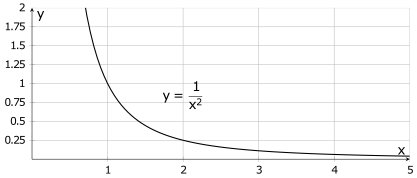
\includegraphics[]{23SQ-Math-1336-Ch8s3-Part1-ws-figure0.png}
%\end{minipage}
%\caption{Graph of \(y=\frac{1}{x^2}\) on the interval from \(x=0\) to \(x=5\)}
\end{figure}


Now show that the improper integral \(\int_1^\infty \frac{dx}{x^2}\) converges, and by the Integral Test, so does \(\sum_{n=1}^\infty \frac{1}{n^2}\).\\

\pagebreak

\item Use an area argument, referencing the figure shown below, to convince yourself that
\[
1+\int_1^\infty \frac{dx}{x} > \sum_{n=1}^\infty \frac{1}{n}
\] 

\begin{figure}[h]
%\begin{minipage}{\textwidth}
%\begin{tikzpicture}
%\begin{axis}[
%	y= 2cm,
%    x=2cm,
%	axis x line=middle,
%	axis y line = middle,
%	ymin=0,ymax=2,
%	xmin=0,xmax=5,
%    grid=both,
%    xtick={0,1,...,5},
%    ytick={0,.25,...,2},
%    xlabel=\(x\),
%    ylabel=\(y\),
%    tick label style={font=\footnotesize}
%]
%
%\addplot [no marks, black, thick, samples=100, domain=.5:5] {x^(-1)};
%
%\node [above] at (axis cs:  2,.6) {\(y=\frac{1}{x}\)};
%
%\end{axis}
%\end{tikzpicture}
%\end{minipage}
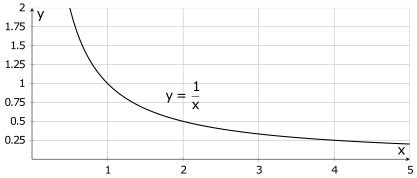
\includegraphics[]{23SQ-Math-1336-Ch8s3-Part1-ws-figure1.png}
%\caption{Graph of \(y=\frac{1}{x}\) on the interval from \(x=0\) to \(x=5\)}
\end{figure}

In one of the pre-class videos, we discovered that the Harmonic Series, \(\sum_{n=1}^\infty \frac{1}{n}\), diverges to \(\infty\).\\
 Use this fact  to argue that \(\int_1^\infty \frac{dx}{x}\) must also diverge.\\



\end{enumerate}

%\pagebreak

\section*{Problems for Group Work:}
\textbf{Be sure to fully justify your reasoning as a part of your solutions.}\\
 The answers are upside-down on the bottom of this page.

\begin{enumerate}

\item Determine the convergence/divergence of the following p-series:

\begin{enumerate} \label{first}
%\begin{multicols}{3}
\item \(\sum_{n=1}^\infty\ \ \frac{1}{n^3}\)

\item \(\sum_{n=1}^\infty\ \ \frac{1}{n^1}\) \label{harm}

\item \(\sum_{n=1}^\infty\ \ \frac{1}{n^{1.00001}}\) \label{00001}
%\end{multicols}
%\item Follow-up question: Why is the convergence behavior different for the series in parts \ref{harm} \& \ref{00001}? In other words, why is \(p=1\) the cutoff between convergence/divergence for p-series?
\end{enumerate}
% Solution: a) Converge, b) Diverge, c) Converge

\vfill


\item If the improper integral \(\int_5^\infty \frac{dx}{x^p}\) converges, which of the following series \underline{must} converge?\label{prob4}
%\begin{multicols}{3}
\begin{enumerate}[A)]
\item \(\sum_{n=1}^\infty \ \frac{1}{n^{p+1}}\)

\item \(\sum_{n=5}^\infty \ \frac{1}{n^{p+1}}\)

\item \(\sum_{n=1}^\infty \ \frac{1}{n^{p-1}}\)

\item \(\sum_{n=5}^\infty \ \frac{1}{n^{p-1}}\)

\item Both A and B

\item Both C and D

\end{enumerate}
%\end{multicols}

\vfill

\item Determine the convergence/divergence of the following series using the tools we currently have: \label{prob3}
\begin{enumerate}[a)]

%\item \(\sum_{n=1}^\infty \ \frac{1}{k^n}, \quad k>1\)\vfill
%
%\item \(\sum_{n=1}^\infty \ \frac{4\cdot 5^n - 5\cdot 4^n}{6^n}\)\vfill
%
%\item \(\sum_{n=1}^\infty \ (-1)^n\)\vfill
%
%\item \(\sum_{n=1}^\infty \ \sin\left(\frac{n}{n+1}\right)\)\vfill
%
%\item \(\sum_{n=1}^\infty \ (-1)^{2n}\)\vfill

\item \(\sum_{n=1}^\infty \ \left[\frac{5}{n(n+1)}-\left(-\frac{1}{2}\right)^n\right]\)\vfill

\item \(\sum_{n=2}^\infty \ \frac{1}{n(\ln n)^p}\)\vfill

\end{enumerate}
%Solution: a) Converge, b) Converge, c) Diverge, d) Diverge, e) Diverge, f) Converge, g) Converge if \(p> 1\), Diverge if \(p\leq 1\)

\end{enumerate}

%\vfill
%\vspace*{-.25in}
%\rotatebox{180}{
%\begin{minipage}{\textwidth}
\subsection*{Answers:}
%\textbf{Problem \ref{prob1}:} a) Diverge, b) Converge to 4, 
%\textbf{Problem \ref{prob2}:} a) Converges to \(\frac{3}{8}\), b) Converges to \(\frac{3}{\pi(\pi-3)}\), 
\textbf{Problem \ref{first}:} a) Converge, b) Diverge, c) Converge
\textbf{Problem \ref{prob4}:} E,\\
\textbf{Problem \ref{prob3}:} a) Converge, b) Converge if \(p> 1\), Diverge if \(p\leq 1\)

%\end{minipage}
%}

\end{document}
